%!TEX root = ../dissertation.tex

\chapter{Experiments}\label{chapt:experiments}

In this chapter, I will describe the experiments we conducted to evaluate our randomized approach to group-oblivious fairness in rankings and compare it to the aforementioned state-of-the-art algorithms, and lay out their results.

\section{Implementation}

All algorithms were implemented in Python. The implementation of ApproximateMultiValuedIPF was the one provided with the original paper. The implementation of DetConstSort was based on the AI Fairness 360 toolkit with minor adjustments.

Sampling from the Mallows distribution was done using the code provided with \cite{fabien2020concentric} at \url{https://github.com/ekhiru/top-k-mallows/}.
All code is available at \url{https://github.com/andrewklayk/fairness_with_mallows_distribution}.

\section{Experimental results}

\subsection{Mallows model and Infeasible Index}\label{exp:exp1}
\label{sec:mallows-ii-exp}
The first experiment aims to evaluate the impact of Mallows randomization on the Infeasible Index of a ranking. The experimental setup and results follow.

\subsubsection{Experiment 1: Setup}
I analyze a scenario of ten candidates, who belong to two equal-sized groups and create multiple rankings, denoted as $\sigma_{II}$, by adjusting the placement of candidates from each group to produce diverse values of the Infeasible Index (II). I then sample rankings from a Mallows distribution using the $\sigma_{II}$ ranking as the central permutation and varying values of $\theta$, observing the resulting Infeasible Index in the samples. 

\subsubsection{Experiment 1: Results} Fig.~\ref{plot:experiment1} shows that as the dispersion parameter increases, the Infeasible Index of samples drawn from Mallows model converges to the Infeasible Index of the central permutation. When the central permutation's Infeasible Index is small, and as  $\theta \rightarrow 0$, the Infeasible Index of the samples drawn from Mallows' model is higher, but without a significant difference. However, when the central permutation's Infeasible Index is large, there is a significant drop in the Infeasible Index of the samples drawn from the Mallows' model as $\theta \rightarrow 0$.

\begin{figure*}[h]
  \centering
  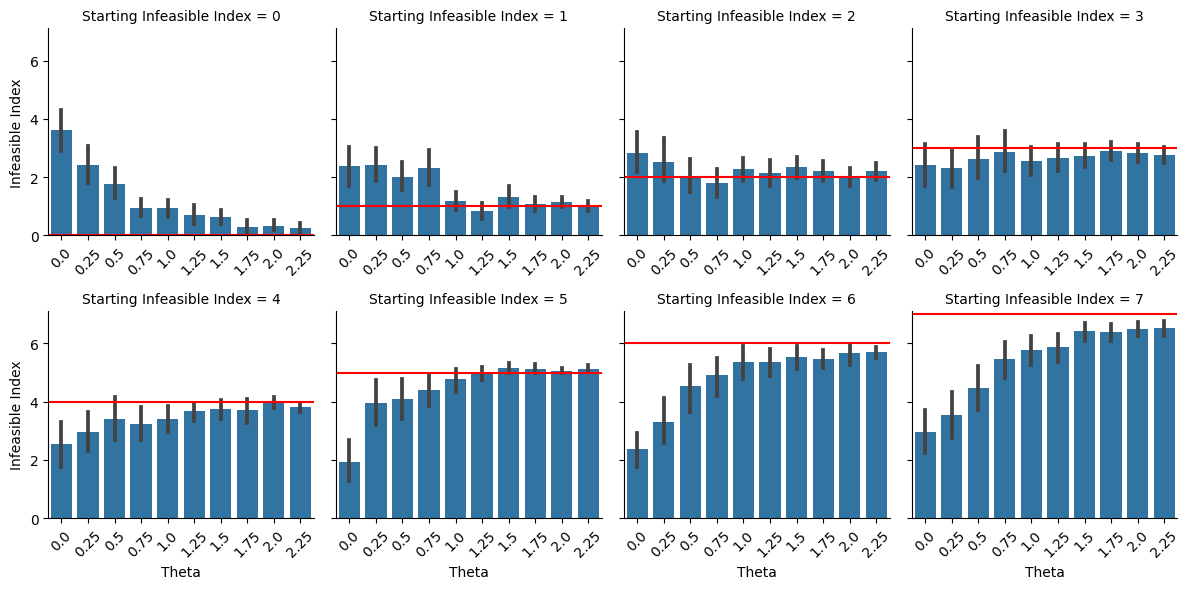
\includegraphics[width=0.8\textwidth]{resources/EXP1_NEW.png}
  \caption{Mallows distribution and Infeasible Index (Experiment 1, Subsection \ref{exp:exp1}). Each subplot corresponds to a different value of the central ranking's Infeasible Index, which is shown as a red line. The bar plots depict the mean value of the Infeasible Index of the samples from the Mallows distribution centered on the initial ranking with two groups. Confidence intervals were obtained via bootstrapping ($n=1000$).}
  \label{plot:experiment1}
\end{figure*}


\subsection{Mallows model and NDCG}\label{exp:exp2}
\label{sec:uniform-exp}
The aim of the second experiment is to evaluate the impact of Mallow's randomization on both fairness and ranking utility in a simple ranking setup.

\subsubsection{Experiment 2: Setup}
I consider two equal-sized groups of five individuals each, where the candidates in the first group are assigned scores $S_1 \sim \mathcal{U}(0,1)$, and the candidates in the second group are assigned scores $S_2 \sim \mathcal{U}(0 + \delta, 1 + \delta)$, where $\delta = \{0.0, 0.1,\dots,0.9,1.0\}$. 
I then sort the candidates according to their descending scores and sample the Mallows distribution centered on the sorted rankings with different values of $\theta$, and evaluate the Infeasible Index and NDCG of the samples.

\subsubsection{Experiment 2: Results} 
Figs. \ref{plot:experiment2infind} and \ref{plot:experiment2ndcg} depict the experimental results in terms of evaluating how the Infeasible Index and the NDCG change as we start from the corresponding Infeasible Index values as depicted in a rankings  Fig. \ref{plot:experiment2initialfairness}. As for the Infeasible Index, we notice similar behavior as in the Fig.~\ref{sec:mallows-ii-exp}. We can see that as the dispersion parameter increases the NDCG converges to that of the central ranking, which is 1. This illustrates that there is a trade-off between the NDCG and the Infeasible Index when sampling from Mallow's distribution with different values of the dispersion parameter.


\begin{figure}[h]
  \centering
  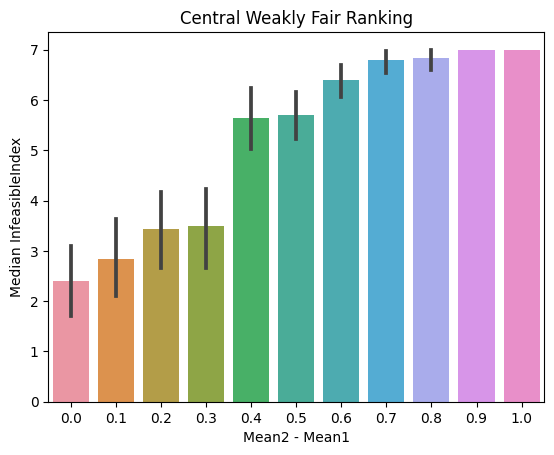
\includegraphics[width=0.4\textwidth]{resources/EXP2_init.png}
  % \caption{Setup of Experiment 2. The Infeasible Index of the Central Ranking and the mean between the score initial ranking is constructed from two groups with scores sampled from two Uniform distributions. The plot shows the Mean Infeasible Index of the initial rankings vs. the difference in means between the score distributions of the two groups. Confidence intervals obtained via bootstrapping ($n=1000$).}
  \caption{The Infeasible Index of the Central Ranking, as constructed by sampling from score distributions for each of the two groups (Experiment 2, Subsection \ref{exp:exp2}). Specifically, the x-axis depicts the difference in means between the score distributions of the two groups. Confidence intervals were obtained via bootstrapping ($n=1000$).}
  \label{plot:experiment2initialfairness}
\end{figure}


\begin{figure}[hp]
  \centering
  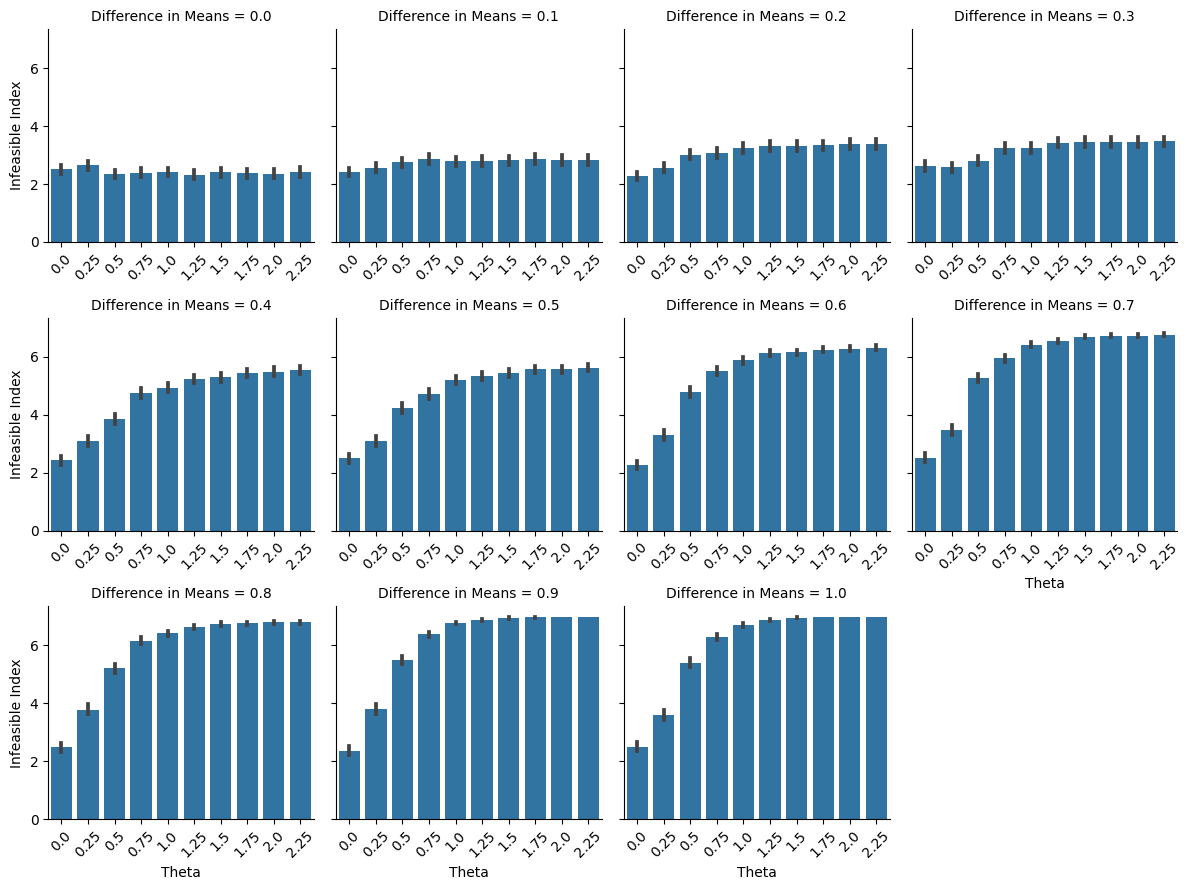
\includegraphics[width=0.6\textwidth]{resources/EXP2_ii_means.png}
  \caption{Mallows distribution and Infeasible Index in a simple score-based ranking setup (Experiment 2, Subsection \ref{exp:exp2}). Each subplot corresponds to a difference in means between the score distributions of the two groups.  We sample five individuals for each group, where the candidates in the first group are assigned scores $S_1 \sim \mathcal{U}(0,1)$, and in the second group - $S_2 \sim \mathcal{U}(0 + \delta, 1 + \delta)$, where $\delta$ is the difference in means. The subplots depict the mean value of the Infeasible Index of the samples from the Mallows distribution centered on the initial ranking. Confidence intervals were obtained via bootstrapping ($n=1000$).}
  \label{plot:experiment2infind}
\end{figure}

\begin{figure}[hp]
  \centering
  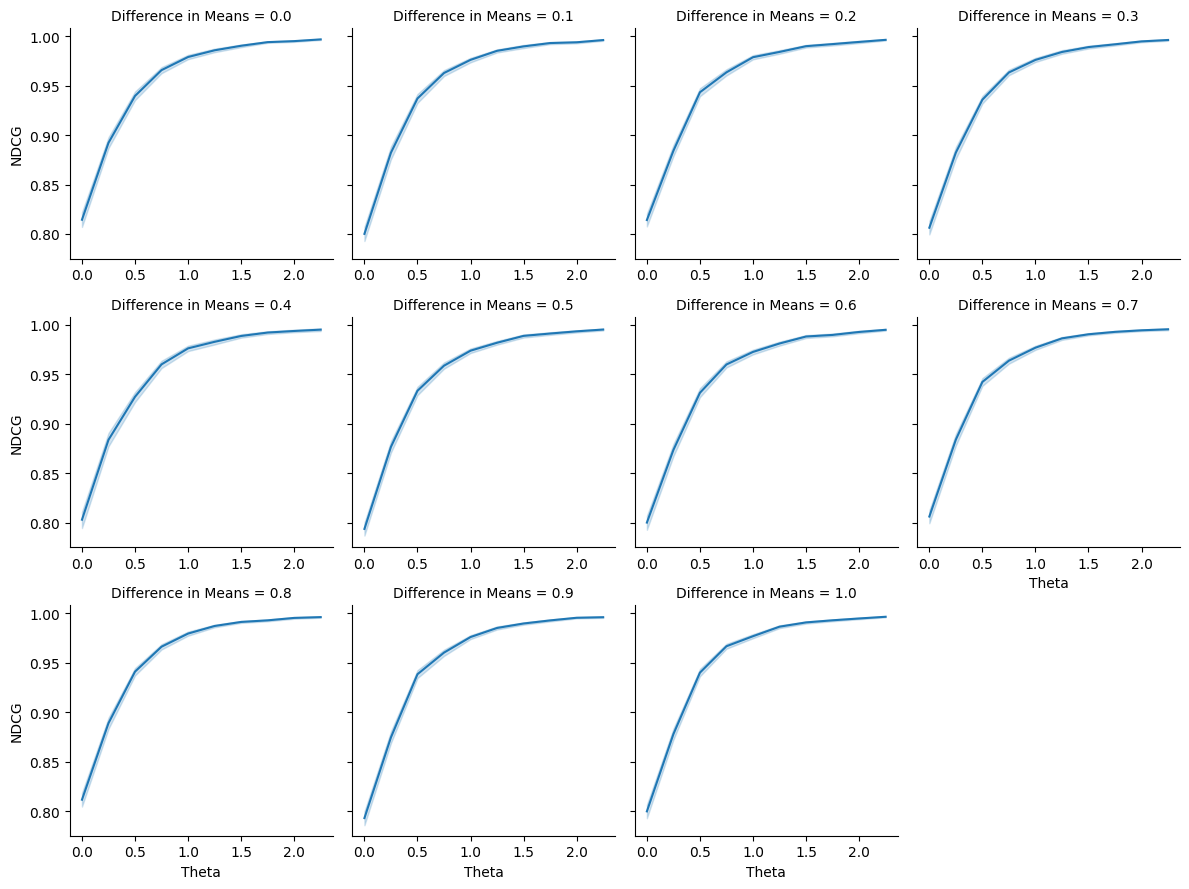
\includegraphics[width=0.6\textwidth]{resources/EXP2_ndcg.png}
  \caption{Mallows distribution and NDCG in a simple score-based ranking setup  (Experiment 2, Subsection \ref{exp:exp2}). Each subplot corresponds to a difference in means between the score distributions of the two groups. We sample five individuals for each group, where the candidates in the first group are assigned scores $S_1 \sim \mathcal{U}(0,1)$, and in the second group - $S_2 \sim \mathcal{U}(0 + \delta, 1 + \delta)$, where $\delta$ is the difference in means. The subplots depict the mean value of NDCG of the samples from the Mallows distribution centered on the initial ranking. Confidence intervals were obtained via bootstrapping ($n=1000$).}
  \label{plot:experiment2ndcg}
\end{figure}


\subsection{A real-world application: German Credit Dataset.}\label{exp:exp3}

In the third experiment, we utilized a real-world dataset to evaluate how well the Mallows randomization method performs in a practical scenario, where we have partial knowledge regarding some of the protected attributes and aim to evaluate the result in terms of an unknown protected attribute. We conduct a thorough experimental analysis with several state-of-the-art postprocessing algorithms that are designed to ensure fairness in rankings regarding specific attributes. To emulate real-world conditions, we introduce noise into their fairness constraints to simulate imperfect knowledge about group membership.

\subsubsection{Dataset Description}
We utilize the German Credit dataset \cite{germancredit}, following the work of \cite{yang2016measuring,RAPF}. For the ranking of the candidates, we use the Credit Amount attribute. 
We aggregate the binary attributes $Sex$ and $Age$ into the $Sex-Age$  protected attribute with four values and consider the information of this attribute as known, with little or no noise. We evaluate the fairness of the algorithms in terms of a third attribute, named $Housing$, with three values. We regarded the $Housing$ attribute as unknown; therefore, it could not be used as information for any algorithm.  The distribution of the groups defined by these attributes is shown in Table~\ref{tab:german_groups}.

\begin{table}[h]
  \centering
\begin{tabular}{ccccc}
\hline
\multicolumn{1}{c}{\multirow{2}{*}{Age-Sex}} & \multicolumn{3}{c}{Housing}                                                     & \multicolumn{1}{l}{\multirow{2}{*}{Total}} \\ \cline{2-4}
\multicolumn{1}{c}{}                         & \multicolumn{1}{l}{free} & \multicolumn{1}{l}{own} & \multicolumn{1}{l}{rent} & \multicolumn{1}{l}{}                       \\ \hline
$<35$ - female                                 & 2                         & 131                      & 80                        & 213                                         \\
$<35$ - male                                   & 23                        & 261                      & 51                        & 335                                         \\
$\geq 35$ - female                             & 17                        & 65                       & 15                        & 97                                          \\
$\geq 35$ - male                               & 66                        & 256                      & 33                        & 355                                         \\ \hline
Total                                          & 108                       & 713                      & 179                       & 1000 \\ \hline                                       
\end{tabular}
   \caption{Distribution of groups defined by Age, Sex, and Housing in the German Credit dataset.}
    \label{tab:german_groups}
\end{table}

\subsubsection{Experiment 3: Setup}

We executed the state-of-the-art ApproxMultiValuedIPF \cite{RAPF}, DetConstSort \cite{linkedin} as well as the ILP algorithm, using as input a weakly-p-fair ranking with respect to the combined $Sex-Age$ protected attribute. The algorithms were run in their vanilla version and with some noisy representation constraints on the combined $Sex-Age$ protected attribute. 
Specifically, we introduced noise into the calculations of the constraints by each of the aforementioned algorithms in the following ways:

\begin{itemize}
    \item ApproxMultiValuedIPF: we added an independent sample from $N(0,\sigma)$ to each of the weights at the weight calculation step ( Algorithm 2, line 2 of \cite{RAPF})
    \item DetConstSort: we added an independent sample from $N(0,\sigma)$ to each of tempMinCounts ( Algorithm 3, line 7 of \cite{linkedin})
    \item ILP: given $X_{ij}, Y_{ij} \sim |N(0,\sigma)|$, we modified the calculation of constraints for each group $G_p$ such that:
    \begin{align*}
    & \lfloor \beta_p \ell \rfloor - X_{ij} \leq \sum_{i \in G_p} \sum_{j = 1}^\ell x_{ij}  \leq \lceil \alpha_p \ell \rceil + Y_{ij} & \forall \ell \in [k]
    \end{align*}
    This was done to lessen the probability of making the problem infeasible, while still retaining noise.
\end{itemize}
We repeated this step 15 times to reliably measure the effect of the noise.

We also run the Mallows algorithm on the same weakly-p-fair ranking, using the weakly-p-fair ranking as a central ranking and dispersion parameters of 0.5 and 1, taking 1 or the best of 15 samples.

We evaluate the fairness of the output rankings using the Infeasible Index with respect to the $Housing$ attribute and the utility of the output rankings using NDCG.
% , as well as the Kendall-Tau distance from the initial weakly-p-fair ranking.
The experiment is repeated for rankings of size {10, 20, 30, 40, 50, 60, 70, 80, 90, 100}.

\subsubsection{Experiment 3: Results}

The experimental results are presented in Figs.~\ref{plot:pfair_hous} and \ref{plot:ndcg}. 
Fig.~\ref{plot:pfair_hous} shows the median percentage of positions satisfying P-fairness with respect to the $Housing$ protected attribute. Since DetConstSort,  ApproxMultiValuedIPF and the ILP use the $Age-Sex$ protected attribute to create the fair ranking, the resulting ranking fairness has to do with another attribute's distribution, therefore we cannot have any guarantees.  For comparison only, we include Fig. \ref{plot:pfair}, so that it is clear how the same ranking can have different fainress scores according to different attribute. We argue that the addition of noise can improve the results regarding different protected attributes, leading to a more balanced output, regardless of the target protected attribute. This approach seems like a compromise among all the different protected attributes that may be present and about which we have no knowledge.

As shown in Fig.~\ref{plot:pfair}, under noisy conditions, the Mallows algorithm performs well compared to state-of-the-art algorithms (DetConstSort and ApproxMultiValuedIPF).
% , which utilize the protected attribute (the subgroups are known).
Fig.~\ref{plot:ndcg} shows the mean NDCG (as a solid line) and a 95\% confidence interval (shaded region). We can notice that as the number of items increase, the NDCG score increases for Mallows, and the performance of the best sample from Mallows approaches the NDCG curve for the ILP.


\begin{figure}
     \centering
     \begin{subfigure}{0.4\textwidth}
         \centering
         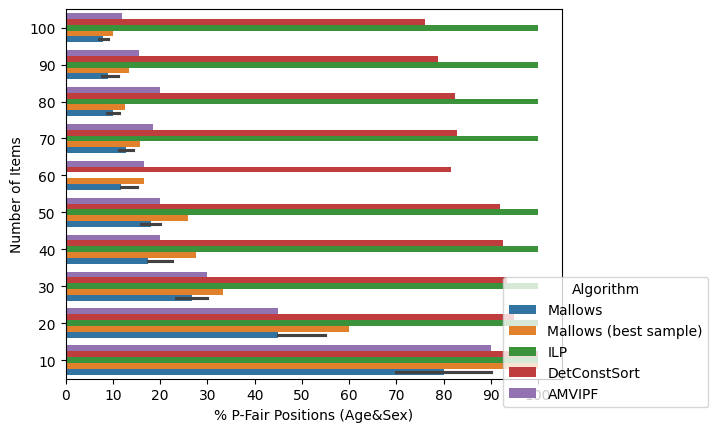
\includegraphics[width=\textwidth]{resources/00/p_pfair.png}
         \caption{$\theta = 0.5$, No noise}
         \label{fig:00pfair}
     \end{subfigure}\quad
     \begin{subfigure}{0.4\textwidth}
         \centering
         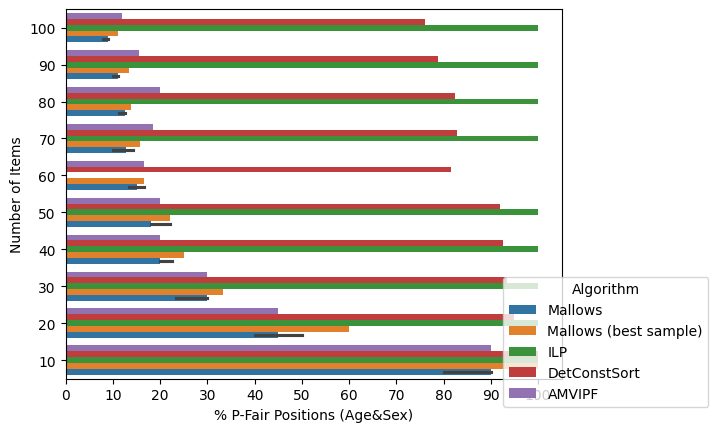
\includegraphics[width=\textwidth]{resources/10/p_pfair.png}
         \caption{$\theta = 1$, No noise}
         \label{fig:10pfair}
     \end{subfigure}\quad
     \begin{subfigure}{0.4\textwidth}
         \centering
         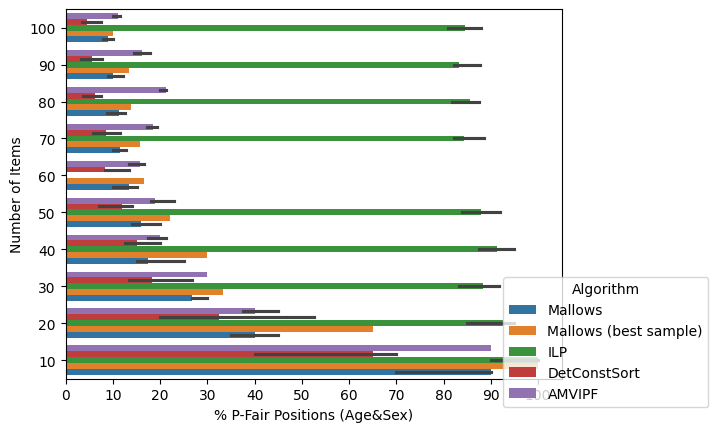
\includegraphics[width=\textwidth]{resources/01/p_pfair.png}
         \caption{$\theta = 0.5, \sigma=1$}
         \label{fig:01pfair}
     \end{subfigure}\quad
     \begin{subfigure}{0.4\textwidth}
         \centering
         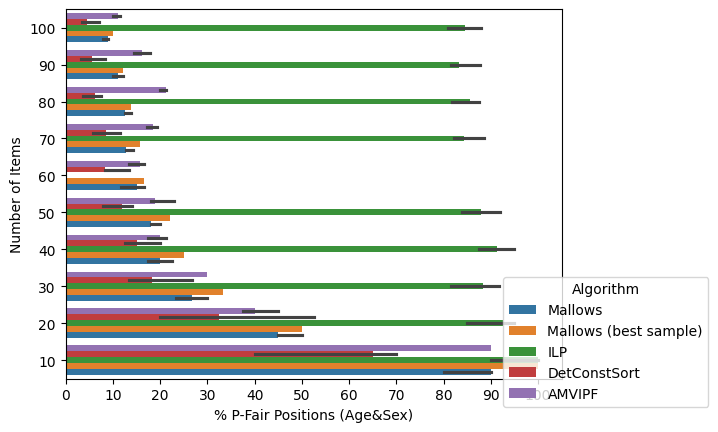
\includegraphics[width=\textwidth]{resources/11/p_pfair.png}
         \caption{$\theta = 1, \sigma=1$}
         \label{fig:11pfair}
     \end{subfigure}\quad
  \caption{ 
  Rankings constructed with noisy representation constraints on the combined $Age-Sex$ protected attribute from an initial weakly-p-fair ranking with respect to the combined $Age-Sex$ protected attribute. \textbf{The plots show the median percentage of positions satisfying P-fairness w.r.t. the $Age-Sex$ protected attribute}. Confidence intervals were obtained via bootstrapping ($n=1000$). In Subfigure (a) the $\theta$ parameter of the Mallows distribution is set to $0.5$, and no noise is added to the constraints. In Subfigure (b) $\theta=1$ and no noise is added to the constraints. In Subfigure (c) $\theta=0.5$ and Gaussian noise $\xi\sim \mathcal{N}(0,1)$ is added to the constraints. In Subfigure  (d) $\theta=1$ and Gaussian noise $\xi\sim \mathcal{N}(0,1)$ is added to the constraints.  
  }
  \label{plot:pfair}
\end{figure}

\begin{figure}
     \centering
     \begin{subfigure}[b]{0.4\textwidth}
         \centering
         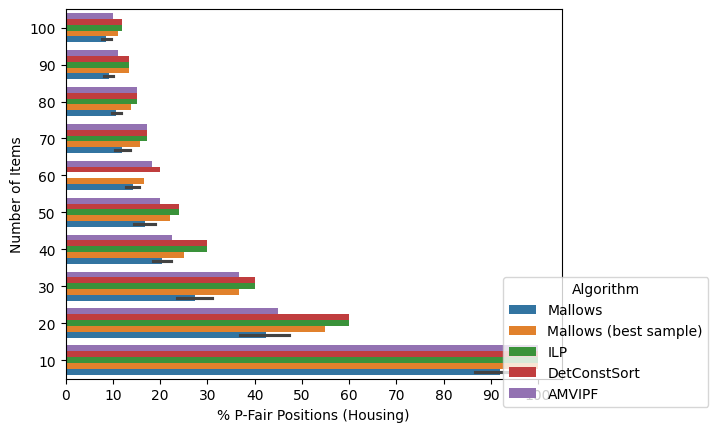
\includegraphics[width=\textwidth]{resources/00/p_pfair_hou.png}
         \caption{$\theta = 0.5$, No noise}
         \label{fig:00pfair}
     \end{subfigure}\quad
     \begin{subfigure}[b]{0.4\textwidth}
         \centering
         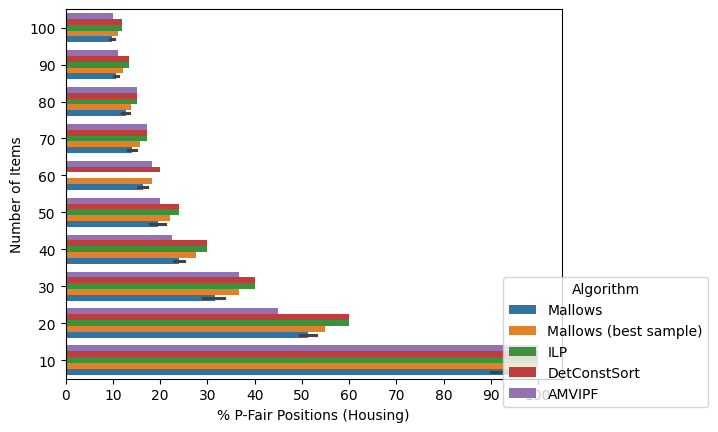
\includegraphics[width=\textwidth]{resources/10/p_pfair_hou.png}
         \caption{$\theta = 1$, No noise}
         \label{fig:10pfair}
     \end{subfigure}\quad
     \begin{subfigure}[b]{0.4\textwidth}
         \centering
         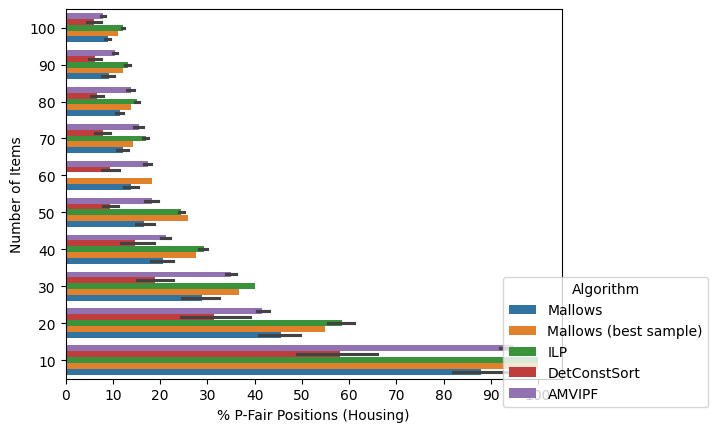
\includegraphics[width=\textwidth]{resources/01/p_pfair_hou.png}
         \caption{$\theta = 0.5, \sigma=1$}
         \label{fig:01pfair}
     \end{subfigure}\quad
     \begin{subfigure}[b]{0.4\textwidth}
         \centering
         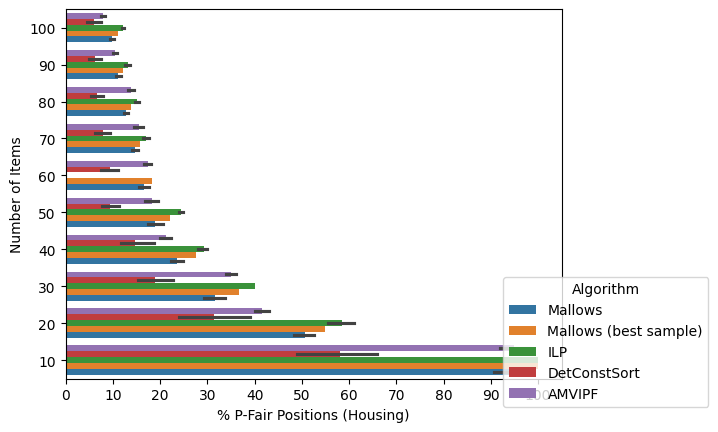
\includegraphics[width=\textwidth]{resources/11/p_pfair_hou.png}
         \caption{$\theta = 1, \sigma=1$}
         \label{fig:11pfair}
     \end{subfigure}\quad
  \caption{ 
  Rankings constructed with noisy representation constraints on the combined $Age-Sex$ protected attribute from an initial weakly-p-fair ranking with respect to the combined $Age-Sex$ protected attribute. \textbf{The plots show the median percentage of positions satisfying P-fairness w.r.t. the $Housing$ protected attribute}. Confidence intervals were obtained via bootstrapping ($n=1000$). In Subfigure (a) the $\theta$ parameter of the Mallows distribution is set to $0.5$, and no noise is added to the constraints. In Subfigure (b) $\theta=1$ and no noise is added to the constraints. In Subfigure (c) $\theta=0.5$ and Gaussian noise $\xi\sim \mathcal{N}(0,1)$ is added to the constraints. In Subfigure  (d) $\theta=1$ and Gaussian noise $\xi\sim \mathcal{N}(0,1)$ is added to the constraints.  
  }
  \label{plot:pfair_hous}
\end{figure}

\begin{figure}
     \centering
     \begin{subfigure}{0.4\textwidth}
         \centering
         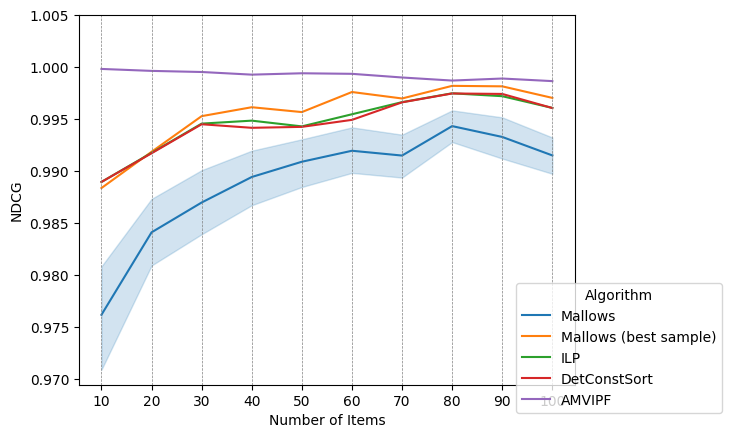
\includegraphics[width=\textwidth]{resources/00/ndcg.png}
         \caption{$\theta = 0.5$, No noise}
         \label{fig:00ndcg}
     \end{subfigure}\quad
     \begin{subfigure}[b]{0.4\textwidth}
         \centering
         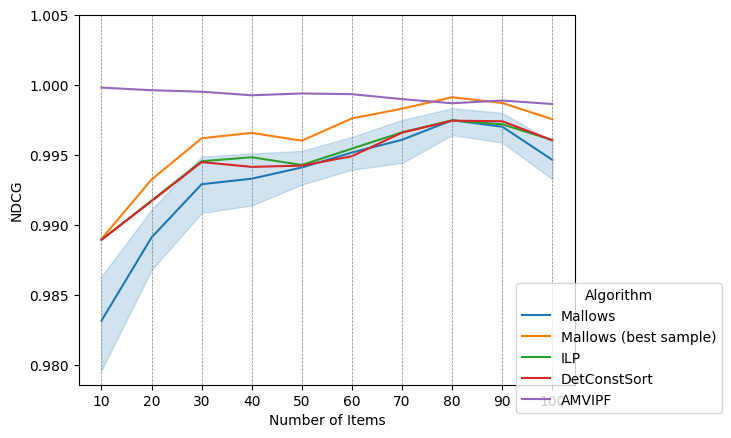
\includegraphics[width=\textwidth]{resources/10/ndcg.png}
         \caption{$\theta = 1$, No noise}
         \label{fig:10ndcg}
     \end{subfigure}\quad
     \begin{subfigure}[b]{0.4\textwidth}
         \centering
         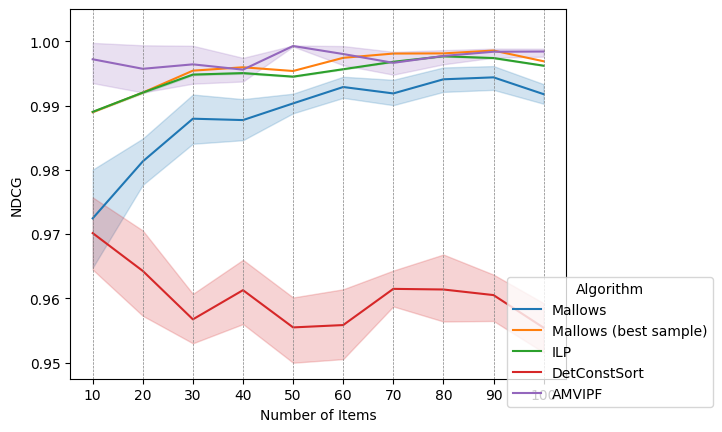
\includegraphics[width=\textwidth]{resources/01/ndcg.png}
         \caption{$\theta = 0.5, \sigma=1$}
         \label{fig:01ndcg}
     \end{subfigure}\quad
     \begin{subfigure}[b]{0.4\textwidth}
         \centering
         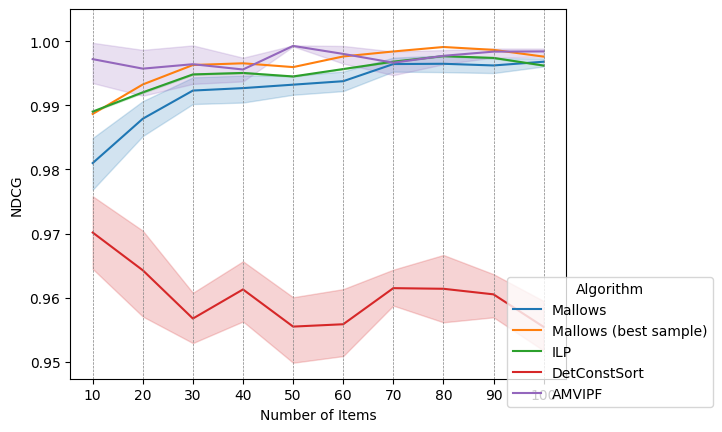
\includegraphics[width=\textwidth]{resources/11/ndcg.png}
         \caption{$\theta = 1, \sigma=1$}
         \label{fig:11ndcg}
     \end{subfigure}\quad
  \caption{
  % Results of Experiment 3:
  Mean NDCG (solid line) and a 95\% confidence interval (shaded region) of the output rankings. Confidence intervals were obtained via bootstrapping ($n=1000$). In Subfigure (a) the $\theta$ parameter of the Mallows distribution is set to $0.5$, and no noise is added to the constraints. In Subfigure (b) $\theta=1$ and no noise is added to the constraints. In Subfigure (c) $\theta=0.5$ and Gaussian noise $\xi\sim \mathcal{N}(0,1)$ is added to the constraints. In Subfigure  (d) $\theta=1$ and Gaussian noise $\xi\sim \mathcal{N}(0,1)$ is added to the constraints.  }
  \label{plot:ndcg}
\end{figure}


